\section{Classical simulation of quantum systems\label{sec:ClassicalSimulationOfQSystems}}

\subsection{Why use classical simulators}

For near-term quantum computers, one might question the necessity of classical simulators to emulate quantum computations. After all, the promise of quantum computing lies in its ability to perform certain tasks exponentially faster than classical computers. However, classical simulators remain invaluable for several compelling reasons \cite{10.1038/s41598-019-47174-9, 9910084,doi.org/10.48550,Fedorov2022unitaryselective,preopt-0,preopt-1,preopt-2,IBMQuantumSummit2023}.

\begin{enumerate}
    \item {\bf Resource Efficiency:} Quantum computer time is a limited and valuable resource. When developing and testing new quantum circuits or algorithms, researchers often need to execute them numerous times to validate their functionality and robustness. Running experiments on a real quantum machine can be time-consuming and costly, particularly when waiting for quantum computer availability after each circuit modification. Classical simulators offer an efficient alternative, allowing researchers to rapidly iterate through experiments without waiting for quantum resources.
    \item {\bf Noise and Error Analysis:} Real quantum machines are susceptible to noise and errors due to environmental factors, making it challenging to control and maintain the desired quantum state fidelity. Classical simulators provide a controlled environment for introducing and analyzing various noise scenarios. Researchers can simulate quantum noises to assess how robust their algorithms are under different conditions, as well as explore error correction techniques. This is a crucial step in building fault-tolerant quantum systems.
    \item {\bf Scalability:} Current quantum machines have limitations in terms of the number of qubits and the noise levels they exhibit. Classical simulators, on the other hand, can be adapted to simulate quantum systems with a larger number of qubits, enabling researchers to explore complex quantum algorithms and states that are beyond the capabilities of existing quantum hardware.
    \item {\bf Versatility:} Classical simulators offer flexibility regarding what they can simulate. Researchers can use them to capture "snapshots" of quantum states during computations, perform measurements, and make decisions based on measurement outcomes. Additionally, they can obtain more comprehensive information, such as the density operator of the system, rather than just specific measurement results.
    \item {\bf Efficiency Trade-Offs:} Building an efficient quantum simulator involves addressing trade-offs between computational efficiency and the range of quantum states it can represent. The choice of simulator depends on the specific needs of the quantum computation being emulated.
    \item {\bf Connectivity:}
    When executing a circuit on quantum hardware, the transpilation step involves mapping logical qubits to physical ones, in a fashion that may one-to-many. This is due to the constraint of the physical connection of qubits, which is not usually all-to-all on true QPUs. When simulating, all qubits can be entangled with all others, thus keeping down the `physical' qubits needed and easing the computational burden of solving the minor-embedding problem.
  \item {\bf Pre-optimization:}
    Variational algorithms can be expensive and require many iterations of a quantum circuit.  Pre-optimization with classical simulators can be used to find approximate circuits parameters that can be used or refined with quantum hardware.\cite{preopt-0,preopt-1,preopt-2}
    \item {\bf HPC-assisted quantum computing:}
    There is a way in which HPC can substantially help to extend the depth of quantum circuits, as demonstrated in the recently developed method called "Operator Backpropagation."~\cite{IBMQuantumSummit2023} The idea is to compute a part of a quantum circuit on a quantum device, and compute the second part of a circuit classically by using a quantum circuit simulator on an HPC system, and then stitch the results together. 
\end{enumerate}
In summary, classical simulators allow for efficient development, testing, and analysis of quantum circuits, algorithms, and states, while also providing a controlled environment for exploring quantum noise and errors. While quantum computers hold immense promise, classical simulators remain a vital component of the quantum computing toolkit, enabling progress and innovation in the field. Furthermore, simulators will likely continue to serve as yet another type of circuit execution environment among multi-node compute clusters for executing distributed workloads, which will be adept at handling (sub-)circuits that fall within their scope.

\subsection{Quantum circuits simulators}

In this section, we describe different types of classical quantum circuit simulators. In particular, we describe their capabilities in terms of what the maximum size systems (in both qubits and gates) that can be simulated using HPC. The advantages and disadvantages of quantum circuit simulators are also discussed, as well as use cases.

Before we start, we note that not every quantum circuit is difficult to simulate on a classical computer. Trivially, a quantum circuit that carries out a purely classical computation is not difficult to simulate on a classical computer. Indeed, some of the quantum circuits that are not difficult to simulate include Clifford circuits~\cite{gottesman1998heisenberg,aaronson2004improved,garcia2014simulation} and the quantum Fourier transform~\cite{aharonov2006quantum,yoran2007efficient}, to name a couple. Some quantum circuits are known to be classically simulable for specific input states as well~\cite{garcia2014simulation}. If the simulation does not need to produce the full spectrum of the output state of a given quantum computation but rather a sampling of such, as it would be the case for obtaining a final, classical result out of a quantum computer upon measurements, the difficulty of the classical simulation can dramatically decrease~\cite{hillmich2020just}. Further decrease in the difficulty is obtained if the simulation is to mimic an error-prone quantum computer executing a quantum circuit~\cite{hillmich2022approximating}. We further note in passing that simulation of a quantum circuit that exhibits sparse couplings between densely connected sets of qubits can be more amenable to classical simulations~\cite{fatima2021faster}, using methodologies not unlike circuit cutting discussed in Sec.~\ref{sec:CNA}.

\subsubsection{State-vector simulators}

State-vector based simulation is to simulate the operations of applying a series of unitary operators $U_{m-1} \cdots U_1 U_0$ to the state-vector representation of the quantum states $\ket{\psi}=\sum_{i=0}^{2^n-1}\alpha_i\ket{i}$, where $n$ is the number of qubits and $m$ is the number of operations or gates. Typically, a complex-valued double or single precision floating-point vector $\vec{\alpha}$ of size $2^n$ is used to store the coefficients $\alpha_i$, which costs $16\times2^n$ bytes of memory for classical simulation. $U_i$ with $i\in[0,m-1]$ is a $2\times2$ (for one-qubit gate) or $4\times4$ (for two-qubit gate) complex matrix. It has been shown that an arbitrary quantum circuit can be decomposed into 1-qubit and 2-qubit gates \cite{barenco1995elementary}. In fact, most quantum devices internally run 1-qubit or 2-qubit basis gates. For example, IBM adopts 1-qubit gate \texttt{X}, \texttt{SX}, \texttt{RZ}, \texttt{ID} and 2-qubit gate \texttt{CX} (recently \texttt{ECR}) as the basis gates. To apply a gate $U$, the operation is $\ket{\psi}\to U\ket{\psi}$. For 1-qubit $U$ applying on qubit $q$ in a quantum register, $\vec{\alpha}$ is updated through the following expression where $s_i=\lfloor i/{2^q}\rfloor 2^{q+1}+(i \% 2^q)$ for every integer $i\in[0, 2^{n-1}-1]$:
\begin{equation}
\begin{bmatrix}
\alpha_{s_i} \\
\alpha_{s_i+2^q}  
\end{bmatrix}
\to
U_{2\times2}\cdot \begin{bmatrix}
\alpha_{s_i} \\
\alpha_{s_i+2^q}  
\end{bmatrix}
\label{eq:1q-op}
\end{equation}
Regarding 2-qubit unitary gate $U$ applying on qubit $p$ and $q$ (assuming $p<q$ without losing generality), $\vec{\alpha}$ is updated  through:
\begin{equation}
\begin{bmatrix}
\alpha_{s_i} \\
\alpha_{s_i+2^p} \\
\alpha_{s_i+2^q} \\
\alpha_{s_i+2^p+2^q}
\end{bmatrix}
\to
U_{4\times4}\cdot \begin{bmatrix}
\alpha_{s_i} \\
\alpha_{s_i+2^p} \\
\alpha_{s_i+2^q} \\
\alpha_{s_i+2^p+2^q}
\end{bmatrix}
\label{eq:2q-op}
\end{equation}
where $s_i{=}\lfloor \lfloor i/{2^p}\rfloor /2^{q-p-1} \rfloor  2^{q+1} + (\lfloor i/{2^p}\rfloor \% 2^{q-p-1})2^{p+1} +  (i \% 2^p)$ for every integer $i\in[0,2^{n-2}-1]$. 

Therefore, state-vector based quantum numerical simulation is to perform a sequence of $2\times2$ or $4\times4$ operations Eq.~(\ref{eq:1q-op}) and Eq.~(\ref{eq:2q-op}) over the large state-vector coefficient array of complex numbers in a classical system.

State vector simulators hold the full coefficients of pure quantum states within the classical system's memory, which scales exponentially with the number of qubits. Consequently, the state vector is often distributed across many nodes of a classical HPC~\cite{haner20170,pednault2017breaking,pednault2019leveraging,li2021sv}. Such simulators however exhibit linear scaling with respect to the circuit depth~\cite{fatima2021faster}. As such, state vector simulations are sensitive to the number of qubits but much less to the gate count or circuit depth. For example, a recent work shows that a low-energy nuclear quantum circuit with 115 million gates on 21-qubits can be effectively simulated within one hour using a GPU for state vector simulation~\cite{li2023deep}.

We note that various forms of approximate state-vector simulators can be tailored to problem specific applications.  For example, recent truncated state vector simulators have been used to simulate VQE for various chemistry problems on 64 qubits without significant loss of accuracy or the need for large computing resources~\cite{preopt-2,approxstatevec}. Combining the state vector simulators with Feynman path summation can trade the circuit depth with the number of qubits or memory usage~\cite{fatima2021faster}, rendering some hard to simulate circuits according to a naive state vector simulator to be simulable due to orders of magnitude improvement in their simulability~\cite{markov2020massively,fatima2021faster}.

\subsubsection{Density matrix simulators}

When dealing with a mixed system where noise is present, a pure state can no longer provide sufficient information about the system. In this case, a mixed state corresponds to a statistical ensemble, or probabilistic mixture of pure states, can be used to describe the condition where a system is entangled with another system, such as the environment from which the noise is imposed. A mixed state is represented by a density matrix or a density operator, which is defined by choosing the basis in the underlying space. The density matrix is given by:
\begin{equation*}
\rho=\sum{p_s\ket{\psi_s}\bra{\psi_s}}
\end{equation*}
where $\rho$ represents the fraction of the ensemble of each pure state and is generally an unknown real value. A density matrix contains all the information of a quantum system, allowing the calculation of the probabilities of the outcomes of any measurement performed.

Compared to state-vector simulation, the density operator requires the conservation of $4^n$ coefficients, where $n$ is the number of eigenstates for each pure state, i.e., the number of qubits. Therefore, the memory cost of a density matrix simulation is $2^n$ times that of a pure state simulation using state-vector. The system also evolves according to the operator or gate sequence. When a particular gate is applied, the density matrix evolves as follows~\cite{li2020density}:
\begin{equation}
\rho(t)=G(t)\rho(0)G(t)^{\dagger}
 \label{eq:onegate}
\end{equation}
where $G(t)$ is the gate at time $t$, and $G(t)^\dagger$ is its adjoint. The evolution of a density matrix is more complicated than that of a state vector, considering the size of $4^n$ and the extra adjoint operator per gate. Although $G(t)$ by itself is a unitary operator, it becomes a general matrix and is not necessarily unitary in the presence of noise. Depending on the noise model, the evolution can become an ensemble of evolutions of corresponding channels, each described by a Kraus operator.

The noisy density matrix quantum numerical simulation is to compute $\rho_\text{out}$ for a n-qubit quantum system, density matrix quantum circuit simulation is to compute $\rho_\text{out}$ for a n-qubit quantum register, given initial state $\rho_\text{in}$ and $m$ non-unitary transformations $G_0$, $G_1$, $\dots$, $G_{m-1}$:
\begin{equation}
 \rho_{\text{out}} = G_{m-1}\cdots (G_1 (G_0 \rho_{\text{in}} G^\dag_0) G^\dag_1)\cdots G^\dag_{m-1}
 \label{eq:dmsim}
\end{equation}
where $G$ and $\rho$ are $2^n\times 2^n$ matrices. Due to noise, $G$ is not necessarily a unitary matrix. $G^\dag$ is the adjoint of $G$ verifying $G^\dag=(G^*)^T$. As real quantum devices typically use 1-qubit or 2-qubit gates representing as $4\times4$ or $16\times16$ matrices, to obtain the matrix $G_i$ with a $2^n\times2^n$ size, Kronecker product or tensor product is used with the identity matrix $I$ for the other qubits. 


\subsubsection{Tensor network simulators}

Quantum tensor networks can be used for the simulation of quantum circuits~\cite{markov2008simulating, lykov2021importance, lykov2021large, lykov2021performance, lykov2022tensor, berquist2022stochastic, shah2023gpu}. These simulators leverage the mathematical framework of tensor networks, which are graphical representations of quantum states and operations, as networks of interconnected tensors. Specifially, the nodes in these networks correspond to tensors, which encode gate operations, while the edges represent indices along which tensors are contracted, reflecting the entanglement and interactions between qubits.

The strength of tensor network simulators lies in their ability to compactly represent quantum states that would otherwise require a prohibitive amount of memory. This is particularly valuable for simulating shallow-depth quantum circuits with a large number of qubits, which are challenging for traditional state-vector simulators. These simulators are still limited by the amount of available distributed memory on a supercomputer. For the current generation of supercomputers, tensor network simulators can run quantum circuits up to approximately 200 qubits without approximations for certain quantum circuits~\cite{lykov2021large}. Larger simulations are possible with a truncated bond dimension as well as other applications with different resource requirements~\cite{preopt-1}.


There are different types of tensor network simulators: Matrix Product States (MPS), Projected Entangled Pair States (PEPS), Tree Tensor Networks (TTN), Multi-scale Entanglement Renormalization Ansatz (MERA), and Continuous Variable Tensor Network (CVTN) to name a few as shown on Figure~\ref{fig:tensornetworks}. MPS is arguably one of the most popular simulators, and it is particularly useful for simulating one-dimensional quantum systems. In MPS, the tensors are arranged in a chain, with each tensor representing the state of a qubit and the connections between them capturing the nearest-neighbor entanglement. One of the MPS applications is an efficient tensor network simulation of lossy Gaussian boson sampling experiments, which has been recently demonstrated \cite{liu2023simulating, Oh2023}.
%{\color{red}Minh: Can we briefly comment on when the other methods (PEPS, TTN, ...) are good?}

\begin{figure}
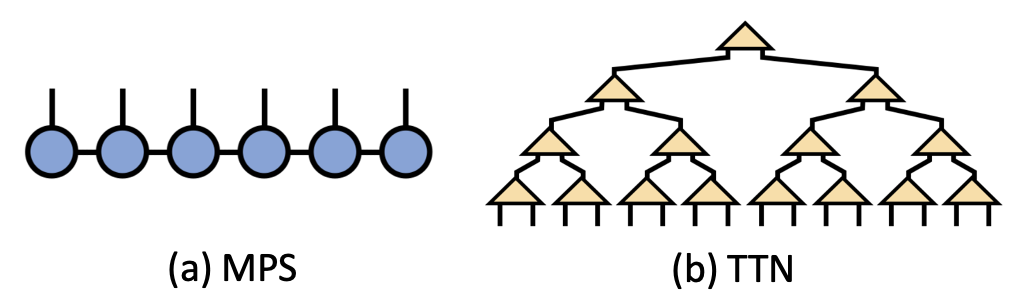
\includegraphics[width=\columnwidth]{groups/3._Classical_simulation_of_quantum_systems/MPS-TTN.png}
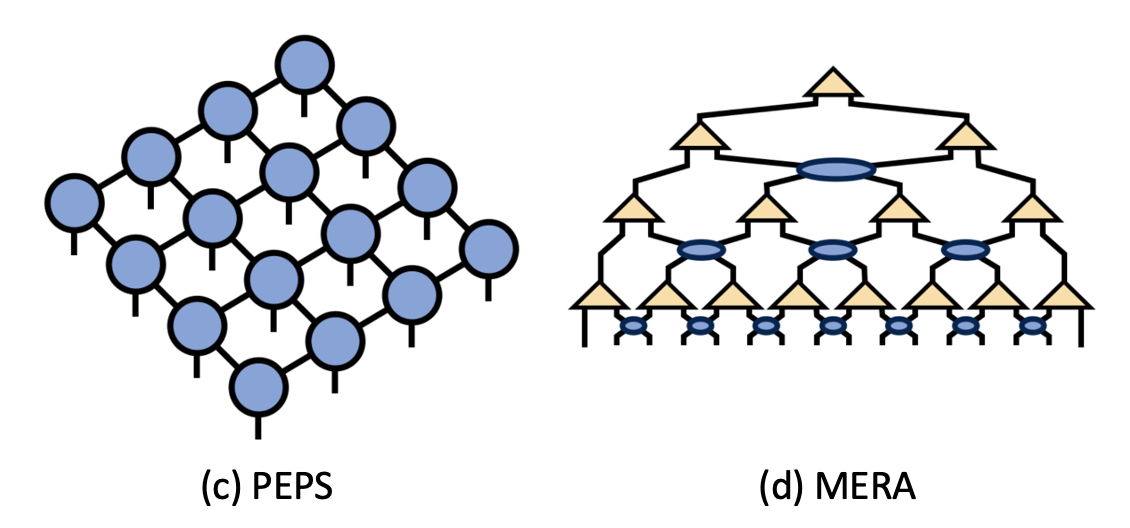
\includegraphics[width=\columnwidth]{groups/3._Classical_simulation_of_quantum_systems/PEPS-MERA.png}
\caption{Different types of tensor network simulators: (a) Matrix Product States (MPS), (b) Tree Tensor Networks (TTN), (c) Projected Entangled Pair States (PEPS), and (d) Multi-scale Entanglement Renormalization Ansatz (MERA).}
\label{fig:tensornetworks}
\end{figure}

Each type of tensor network has its specific applications, advantages, and limitations, and the choice of which to use depends on the application, size, and structure of a quantum circuit:
\begin{itemize}
    
\item MPS simulators excel in one-dimensional quantum systems with short-range interactions. They are efficient for simulating ground and excited states, as well as dynamical properties, due to their ability to capture entanglement in a scalable manner with limited entanglement entropy.

\item  PEPS are generalizations of MPS to higher dimensions, making them suitable for two-dimensional quantum systems. They are adept at handling both short- and long-range interactions, but their computational complexity increases significantly with the system's size and entanglement.

\item  TTN simulators are structured in a hierarchical, tree-like manner, offering efficient computation for certain quantum circuits, especially those with hierarchical or layered structures. They are particularly useful for simulating states that exhibit hierarchical entanglement patterns and for providing insights into quantum many-body systems.

\item  MERA is designed for critical systems with long-range entanglement. It excels in representing ground states of quantum many-body systems near criticality, offering insights into scaling and universality in quantum phase transitions.

\item  CTVN simulators are tailored for quantum systems with continuous variables, like quantum fields or modes of light. They are adept at handling systems where particle number isn't conserved and are crucial in studying non-Gaussian states and processes in quantum optics and field theories.
\end{itemize}

Tensor network simulators continue to evolve, with ongoing research aimed at increasing their efficiency, scalability, and applicability to a broader range of quantum computing tasks.


\subsubsection{Open system Lindblad quantum simulators}

Open-system Lindblad quantum simulators are specifically designed to model the dynamics of quantum systems interacting with external environments. The applications include, for example, simulating quantum magnetism, topological materials, 
quantum phase transitions, and electron transportation. Unlike closed quantum systems, open systems are subject to environmental influences that lead to non-unitary processes such as decoherence and dissipation. These simulators leverage the Lindblad master equation, which blends the unitary evolution dictated by the system's Hamiltonian with the non-unitary aspects resulting from environmental interactions. This approach allows for a comprehensive simulation of open quantum systems, capturing the complexity of quantum noise and the environmental effects. Recently, a novel approach, called noisy quantum gates, has been proposed, as a classical simulation of the Lindblad dynamics~\cite{noisygates}. It is based on integrating the noise into the gates, rather than keeping gates and noise as two separate dynamics, an approach can be generalized to non-Markovian dynamics by using colored noises.

In general, there are a few ways to formulate, but the most common is to use the density matrix formalism, which is adept at representing mixed states, a critical aspect when dealing with open systems. These simulators provide researchers with the flexibility to define specific system-environment interactions, making them a versatile tool across various quantum research domains, especially in material science applications. Its ability to accurately model quantum noise induced by the environment is an especially valuable aspect of it. Overall, the open-system Lindblad quantum simulators stand as a very valuable tool in quantum research, enabling a deeper understanding of the environmental impacts on quantum systems and aiding in the advancement of practical quantum applications.


\subsection{Overview of classical simulators}

In summary, we described four main types of quantum circuit simulators. In the context of material science, the choice of a quantum circuit simulator depends on the specific characteristics of the system under study and the phenomena of interest. Here is how each type of simulator can be used:

State-vector simulators are ideal for systems that can be accurately represented by pure quantum states. In material science, they are particularly useful for studying the evolution of quantum states under Hamiltonians with relatively few degrees of freedom. They excel in scenarios where the full quantum state needs to be tracked, such as in the simulation of small, isolated quantum systems or systems with limited entanglement.

Density matrix simulators are well suited for studying systems where mixed states are prevalent, which includes most real-world scenarios in material science. They can handle decoherence and other noise effects, making them suitable for simulating open quantum systems or systems under non-ideal conditions. Density matrix simulators are ideal for investigating phenomena in quantum materials where environmental interactions play a significant role.

Different types of tensor network simulators have different use cases.
MPS and TTN are powerful in simulating one-dimensional and certain hierarchical quantum systems, respectively. They can efficiently model systems with short-range interactions, which are common in material science. These simulators are especially useful for studying ground state properties and low-energy excitations in materials.
PEPS and MERA are more suited for higher-dimensional systems. PEPS can handle both short- and long-range interactions in two-dimensional materials, making them valuable for exploring complex quantum materials, such as high-temperature superconductors. MERA is particularly effective in studying critical phenomena and phase transitions in materials.

Open system Lindblad quantum simulators are designed to handle non-unitary evolution, which is typical in open quantum systems, where the system is in contact with an external environment. In material science, they are crucial for studying decoherence, dissipation, and thermalization processes in materials. Lindblad simulators are particularly relevant for investigating quantum materials and devices operating under realistic, non-ideal conditions, where environmental interactions cannot be ignored. They are essential for understanding the behavior of materials in quantum information processing and quantum sensing applications, where control and mitigation of decoherence are critical.

Using HPC is critical for simulating large quantum circuits. Ultimately, supercomputers can simulate relatively small quantum circuits because of the exponential requirement of available distributed memory. The next generation of quantum simulators will probably use small quantum computers to simulate very large quantum circuits. The idea is to use small quantum computers to perform tasks that are inherently quantum in nature, such as the contraction of intermediate multi-dimensional tensors, which are central to tensor network simulations. This idea is closely related to Feynman's proposal to use quantum computers to simulate quantum systems~\cite{hey2018feynman}. One way is to use Harrow-Hassidim-Lloyd (HHL) algorithm for the contraction of very high-dimension tensors, which is currently a bottleneck of classical tensor network simulators. The HHL algorithm can be adapted to perform tensor contractions by encoding the tensors as linear systems. This could potentially revolutionize tensor network simulations by dramatically reducing the computational complexity of these contractions. This approach promises a scalable pathway for quantum simulation, as improvements in quantum hardware, such as increased qubit counts and enhanced coherence times, would directly translate into an increased capacity for simulating larger and more complex quantum circuits.

\iffalse
\subsection{Simulation of time dynamics} 
Move to another section.

People: Yuri Alexeev, Burns Healy, Bo Phang, Niri Govind

Describe here the challenges of simulating time dynamics classically and make the case for quantum simulations. Cover topics such as simulation of quantum effects, scalability, and accuracy.

Write text on Yang-Baxter circuit compression. Describe how to perform these calculations efficiently and the challenges for achieving quantum advantage.

The time evolution of quantum systems described by Ising-type Hamiltonians is a very important problem in condensed matter physics and quantum information. These Hamiltonians encompass a wide range of physical phenomena, from magnetic interactions in condensed matter systems to the formulation of optimization problems for quantum computing. In particular, the Ising model describes a lattice of spins with pairwise interactions, characterized by a Hamiltonian that depends on the arrangement of spins and the interaction strengths between them. The general form of an Ising-type Hamiltonian is given by:

\begin{equation}
H = -\sum_{i, j} J_{ij}(t) \sigma_i \sigma_j - \sum_{i} h_i(t) \sigma_i,
\label{ising_hamiltonian}
\end{equation}

where $\sigma_i^z$ and $\sigma_i^x$ represent Pauli matrices, $J_{ij}(t)$ are time-dependent coupling strengths, $h_i(t)$ are time-dependent magnetic fields, and the summations extend over all pairs of spins and single-spin terms.

The problem of accurate large-scale time dynamics simulations remains an area of active research. List the challenges (noise, size, time dynamics length) and opportunities.


\subsection{Simulation of ground states}

Quantum Monte Carlo, etc. 

\subsection{Simulation of finite-temperature systems}

\fi







